\section{VideoQA Reformulation}
\label{sec:reformulation}

\wx{Here we argue that disclosing ``Which part of the video is critical to answering the question?'' is the key to presenting the visual-linguistic alignment explicitly.
To this end, we take a causal \cite{pearl2009causal} look at the reasoning process of VideoQA, then formalize it as a Structure Causal Model (SCM) \cite{pearl2016causal} by investigating the causal relationships among five variables: input video $V$, question $Q$, causal scene $C$, environment scene $E$, ground-truth answer $A$.
% Moreover, we analyze the conventional ERM scheme's limitations on
}

% Discovering the grounding rationale for faithful prediction requires careful inspection of the data generating process. In light of the causal theory \cite{pearl2016causal}, we revisit the formation of VideoQA models, then formalize them as a Structure Causal Model (SCM) \cite{pearl2009causal}  by investigating causality among five variables: input video $V$, question $Q$, causal scene $C$, environment scene $E$, ground-truth answer $A$.

\subsection{Causal Graph of VideoQA}\label{sec:causal-view}
\wx{Figure \ref{fig:scm} illustrates the causal graph, where each link depicts the cause-effect relationship between two variables:
\begin{itemize}[leftmargin=*]
    \item $Q\to C, E \gets V$. Given the question of interest $Q$, the video $V$ can be partitioned into two parts: (1) the causal scene $C$, which retains the question-critical information and naturally serves as the rationale for answering, (2) the environment scene $E$, which gathers the cues irrelevant to the question-answering. For example, to answering ``What is the girl doing?'' in Figure \ref{fig:overview}, $C$ should be the first two clips describing the ``girl-riding on-horse'' scene, while $E$ should be the last clip about the ``meadow'' scene. Moreover, the varying semantics of different questions will emphasize different $C$.
    \item $Q\rightarrow A \leftarrow C$. The visual knowledge in the causal scene $C$ and the linguistic semantics in the question $Q$ collaborate together to determine the answer $A$. Furthermore, this path, which presents the visual-linguistic alignment, internally interprets the reasoning.
    \item $E\dashleftarrow\dashrightarrow C$. The dashed arrow sketches additional probabilistic dependencies \cite{reason:Pearl09a} between $C$ and $E$, which typically arise from selection bias \cite{DBLP:conf/cvpr/TorralbaE11}. For example, the ``meadow'' scene is frequently collected as a common environment for the ``horse-riding'' scene. 
\end{itemize}}


\subsection{Beyond ERM}
\lyc{With inspections on prior VideoQA studies, we investigate their inability to distinguish the causal and non-causal effects of scenes.
Specifically, in conventional VideoQA models, video and question are directly paired together to model their interaction and approach the golden answer, consequently.
Inevitably, taking video as a whole leaves the contributions of scenes untouched, thus failing to differentiate $C$ from $E$ and forgoing their function divergence towards the answer.
Worse still, ERM enforces these models to blindly capture the statistical correlations between the video-question pairs and answers.
As such, the visual-linguistic alignment hinges easily on the spurious correlations between $E$ and $A$, owing to the backdoor paths \cite{pearl2016causal}, which hinders the generalization of models \cite{niu2020counterfactual,wu2022dir}.
Therefore, identifying the causal scene $C$ is the critical to addressing these limitations.}



\begin{figure}[t]
\centering
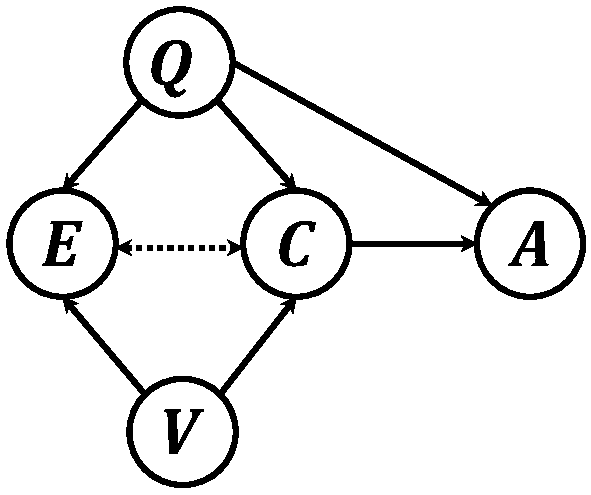
\includegraphics[scale=0.3]{fig/scm.pdf}
\vspace{-5pt}
\caption{Causal Graph of VideoQA}
\vspace{-10pt}
\label{fig:scm}
\end{figure}
